\documentclass[../main.tex]{subfiles}
\begin{document}
\paragraph{Online solutions}\label{par:burgers_rom}

The ROM is spanned by $N_{r}=22$ POD-basis functions in order to retain $99\%$ of the energy of the FOM (see Figure \ref{fig:burgers_decay}).
This is significantly higher than the linear hyperbolic cases in subsection \ref{subsubsec:conservation} thus highlighting the slow decay of the singular values for nonlinear advection-dominated models.

\begin{figure}[H]
    \centering 
    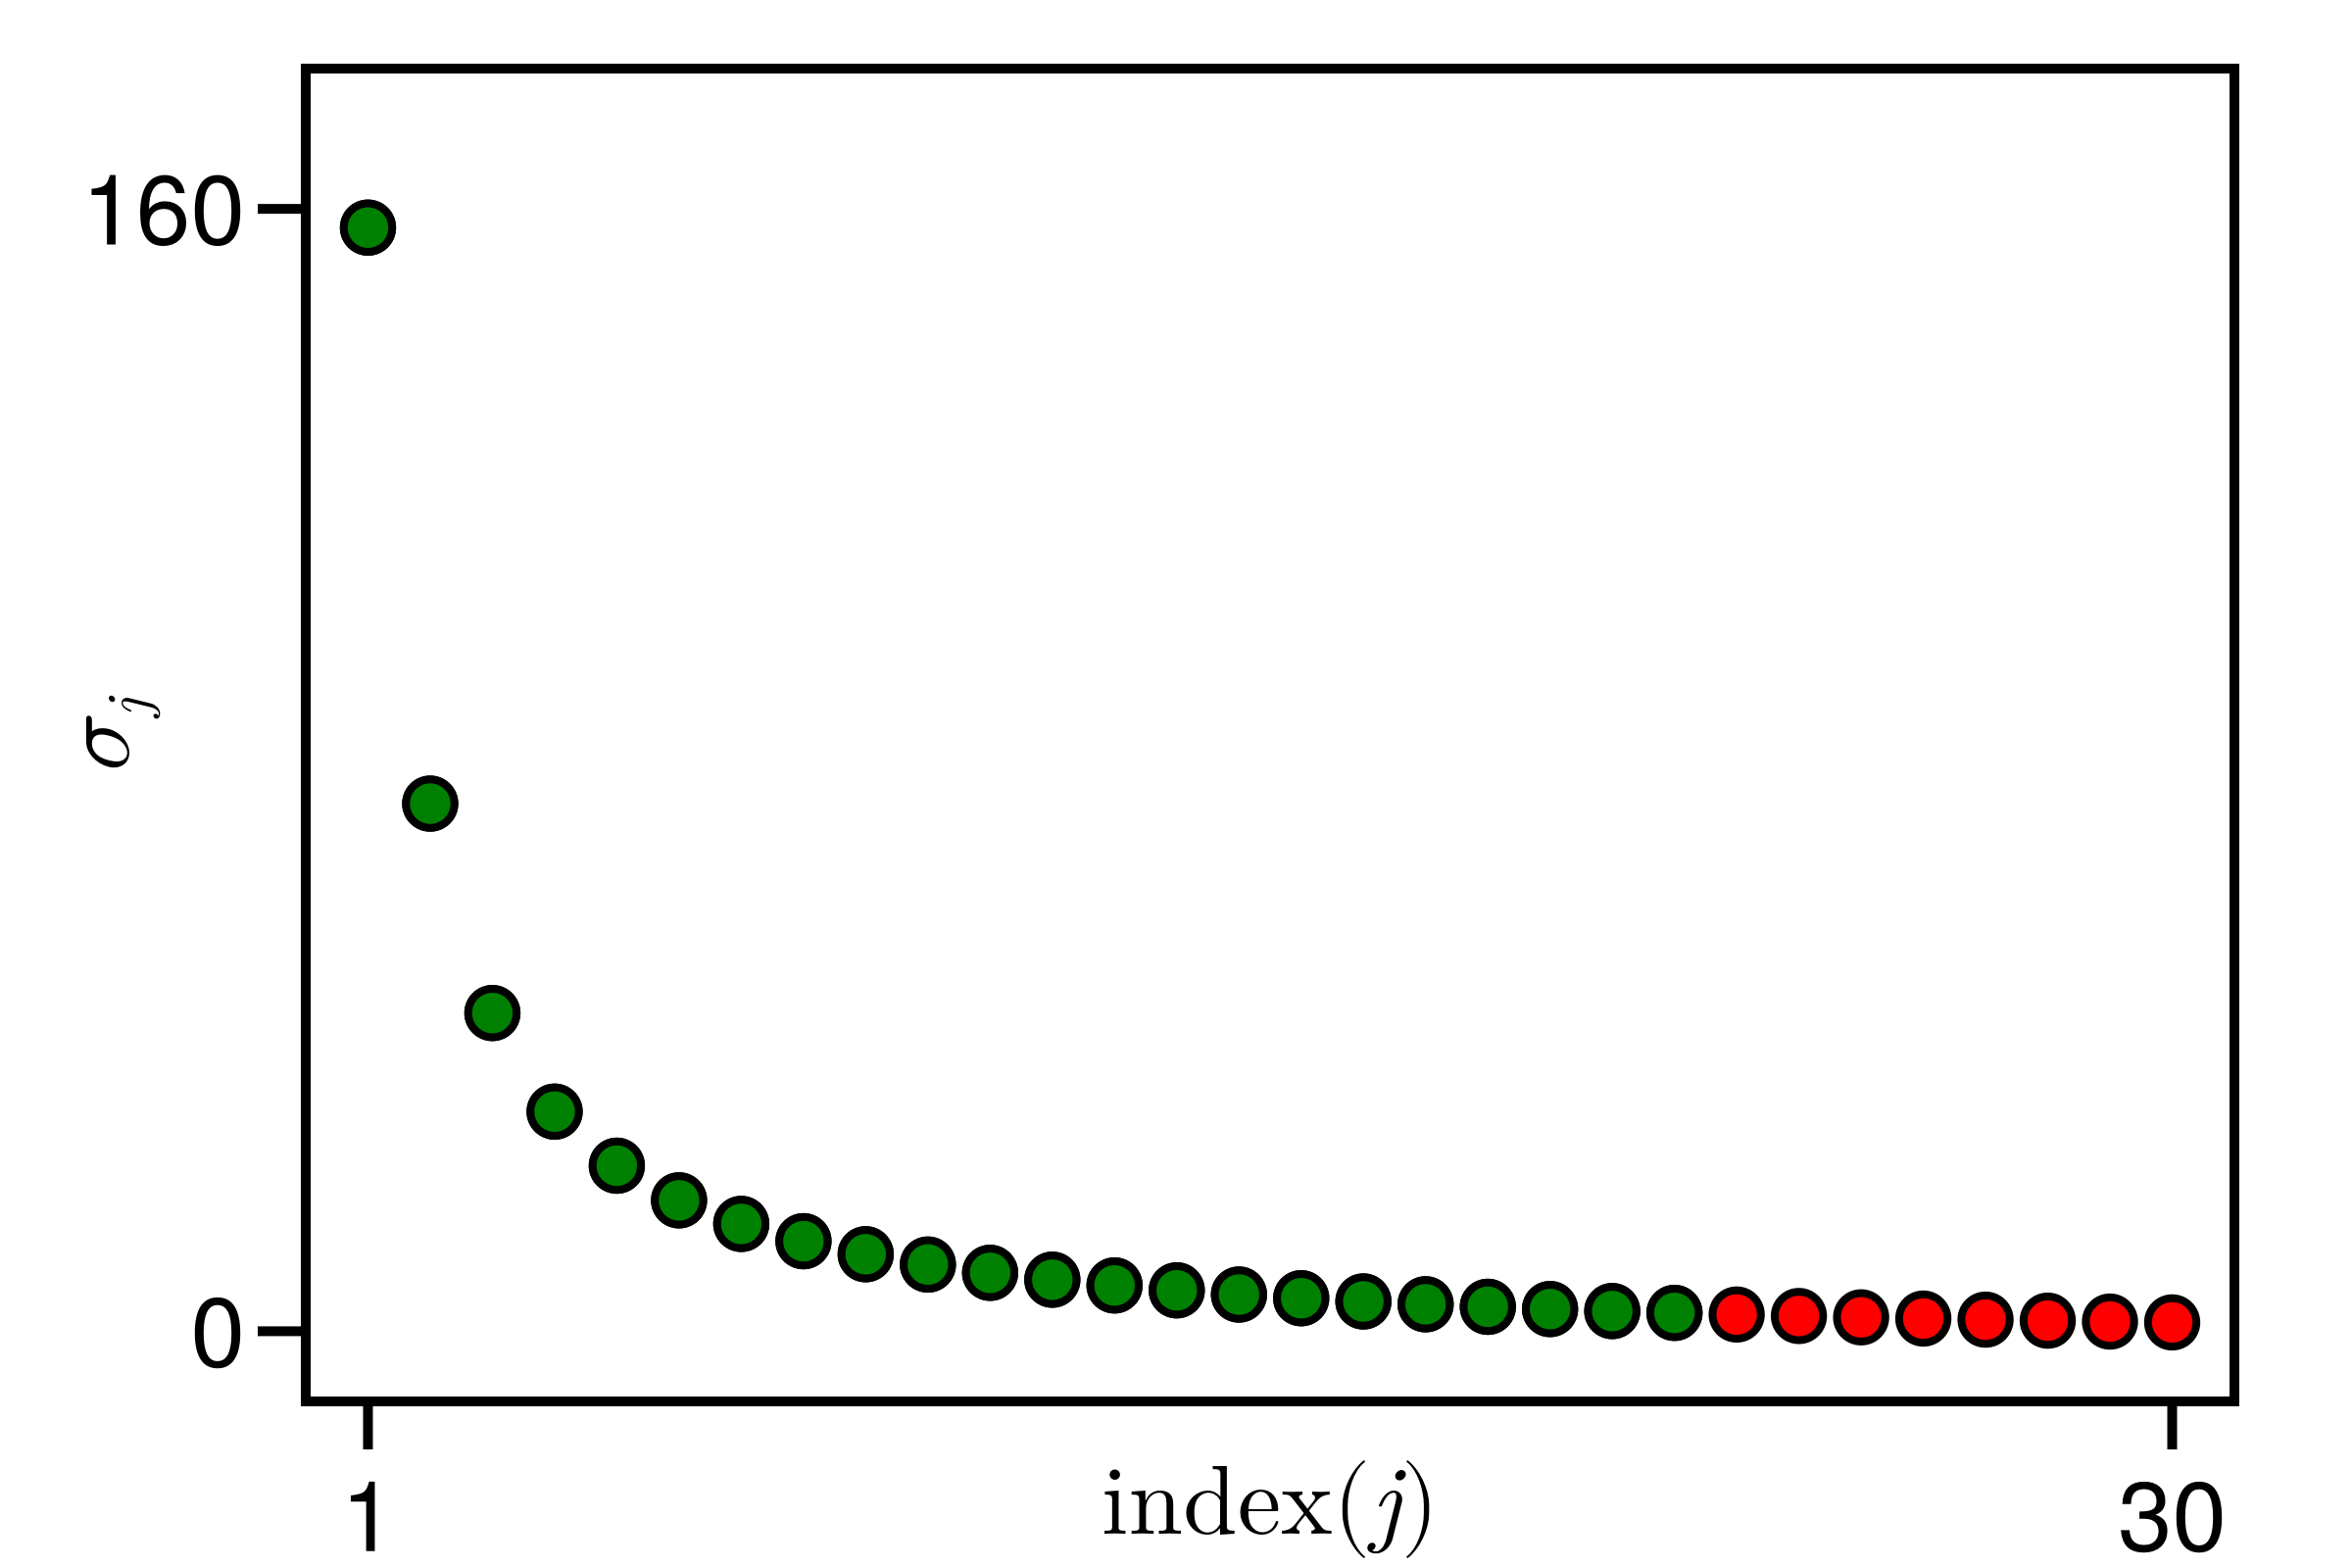
\includegraphics[keepaspectratio, width=0.7\textwidth]{../figures/fig:burgers_decay.png}
    \caption{Kolmogoroff $n-$width decay of \eqref{eq:burgers}. Green dots represent the $N_{r}=22$ singular values used for constructing $\mathcal{R}_{h}$.}
    \label{fig:burgers_decay}
\end{figure}

The reconstruction of the reduced solution will now follow the entirety of the procedure outlined in \eqref{eq:reduced_dynamical_system} (Galerkin projection of the time-dependent FOM onto $\mathcal{R}_{H}$) due to the presence of the nonlinear term. 
The evolution equation for the reduced coefficients will thus be

\begin{equation*}
        \dot{\bar{\boldsymbol{u}}} = \boldsymbol{L}_{r}\bar{\boldsymbol{u}} - \boldsymbol{c}_{r} \,,
\end{equation*}

where $\boldsymbol{L}_{r} = \boldsymbol{V}_{r}^{T}\boldsymbol{L}\boldsymbol{V}_{r}$ is the reduced (linear) operator $\boldsymbol{L}=\boldsymbol{M}^{-1}\boldsymbol{D}$ and $\boldsymbol{c}_{r}(\boldsymbol{u}_{h}) = \boldsymbol{V}_{r}^{T}\boldsymbol{c}(\boldsymbol{u}_{h})$ is the reduced (nonlinear) advection $\boldsymbol{c}(\boldsymbol{u}_{h})=\boldsymbol{M}^{-1}\boldsymbol{N}(\boldsymbol{u}_{h})$.
In order to evaluate the nonlinear term $\boldsymbol{c}_{r}$ we first use the FOM $\boldsymbol{u}_{h}(\mu=\mu^{*})$ to compute $\boldsymbol{N}(\boldsymbol{u}_{h}(\mu^{*}))$ and then we project it onto $\mathcal{R}_{h}$ by multiplying it by $\boldsymbol{V}_{r}^{T}$ from the left.
This \textit{non-intrusive} is computationally expensive as it requires the solution of the full-order system.
Using Euler implicit timestepping we set up a reduced $0-$problem similar to \eqref{eq:burgers_fom} which results in

\begin{equation}\label{eq:burgers_rom}
        \delta t \boldsymbol{V}_{r}^{T}\boldsymbol{c}(\boldsymbol{u}_{h}(t_{n+1})) + (\delta t \boldsymbol{L}_{r} - \boldsymbol{I})\bar{\boldsymbol{u}}(t_{n+1}) - \bar{\boldsymbol{u}}(t_{n}) =: \boldsymbol{G}_{r}(\bar{\boldsymbol{u}}) = \boldsymbol{0}_{\mathbb{R}^{N_{r}}} \,.
\end{equation}

Notice how the nonlinearity in the advection field has severly complicated the ROM \eqref{eq:burgers_rom} as it now requires full-order evaluations at the online stage in order to represent the evolution of $\boldsymbol{u}_{h}$ in $\mathcal{R}_{h}$.
Some of these solutions (compared with those at full-order) are reported in Figure \ref{fig:burgers_rom} below

\begin{figure}[H]
    \centering 
    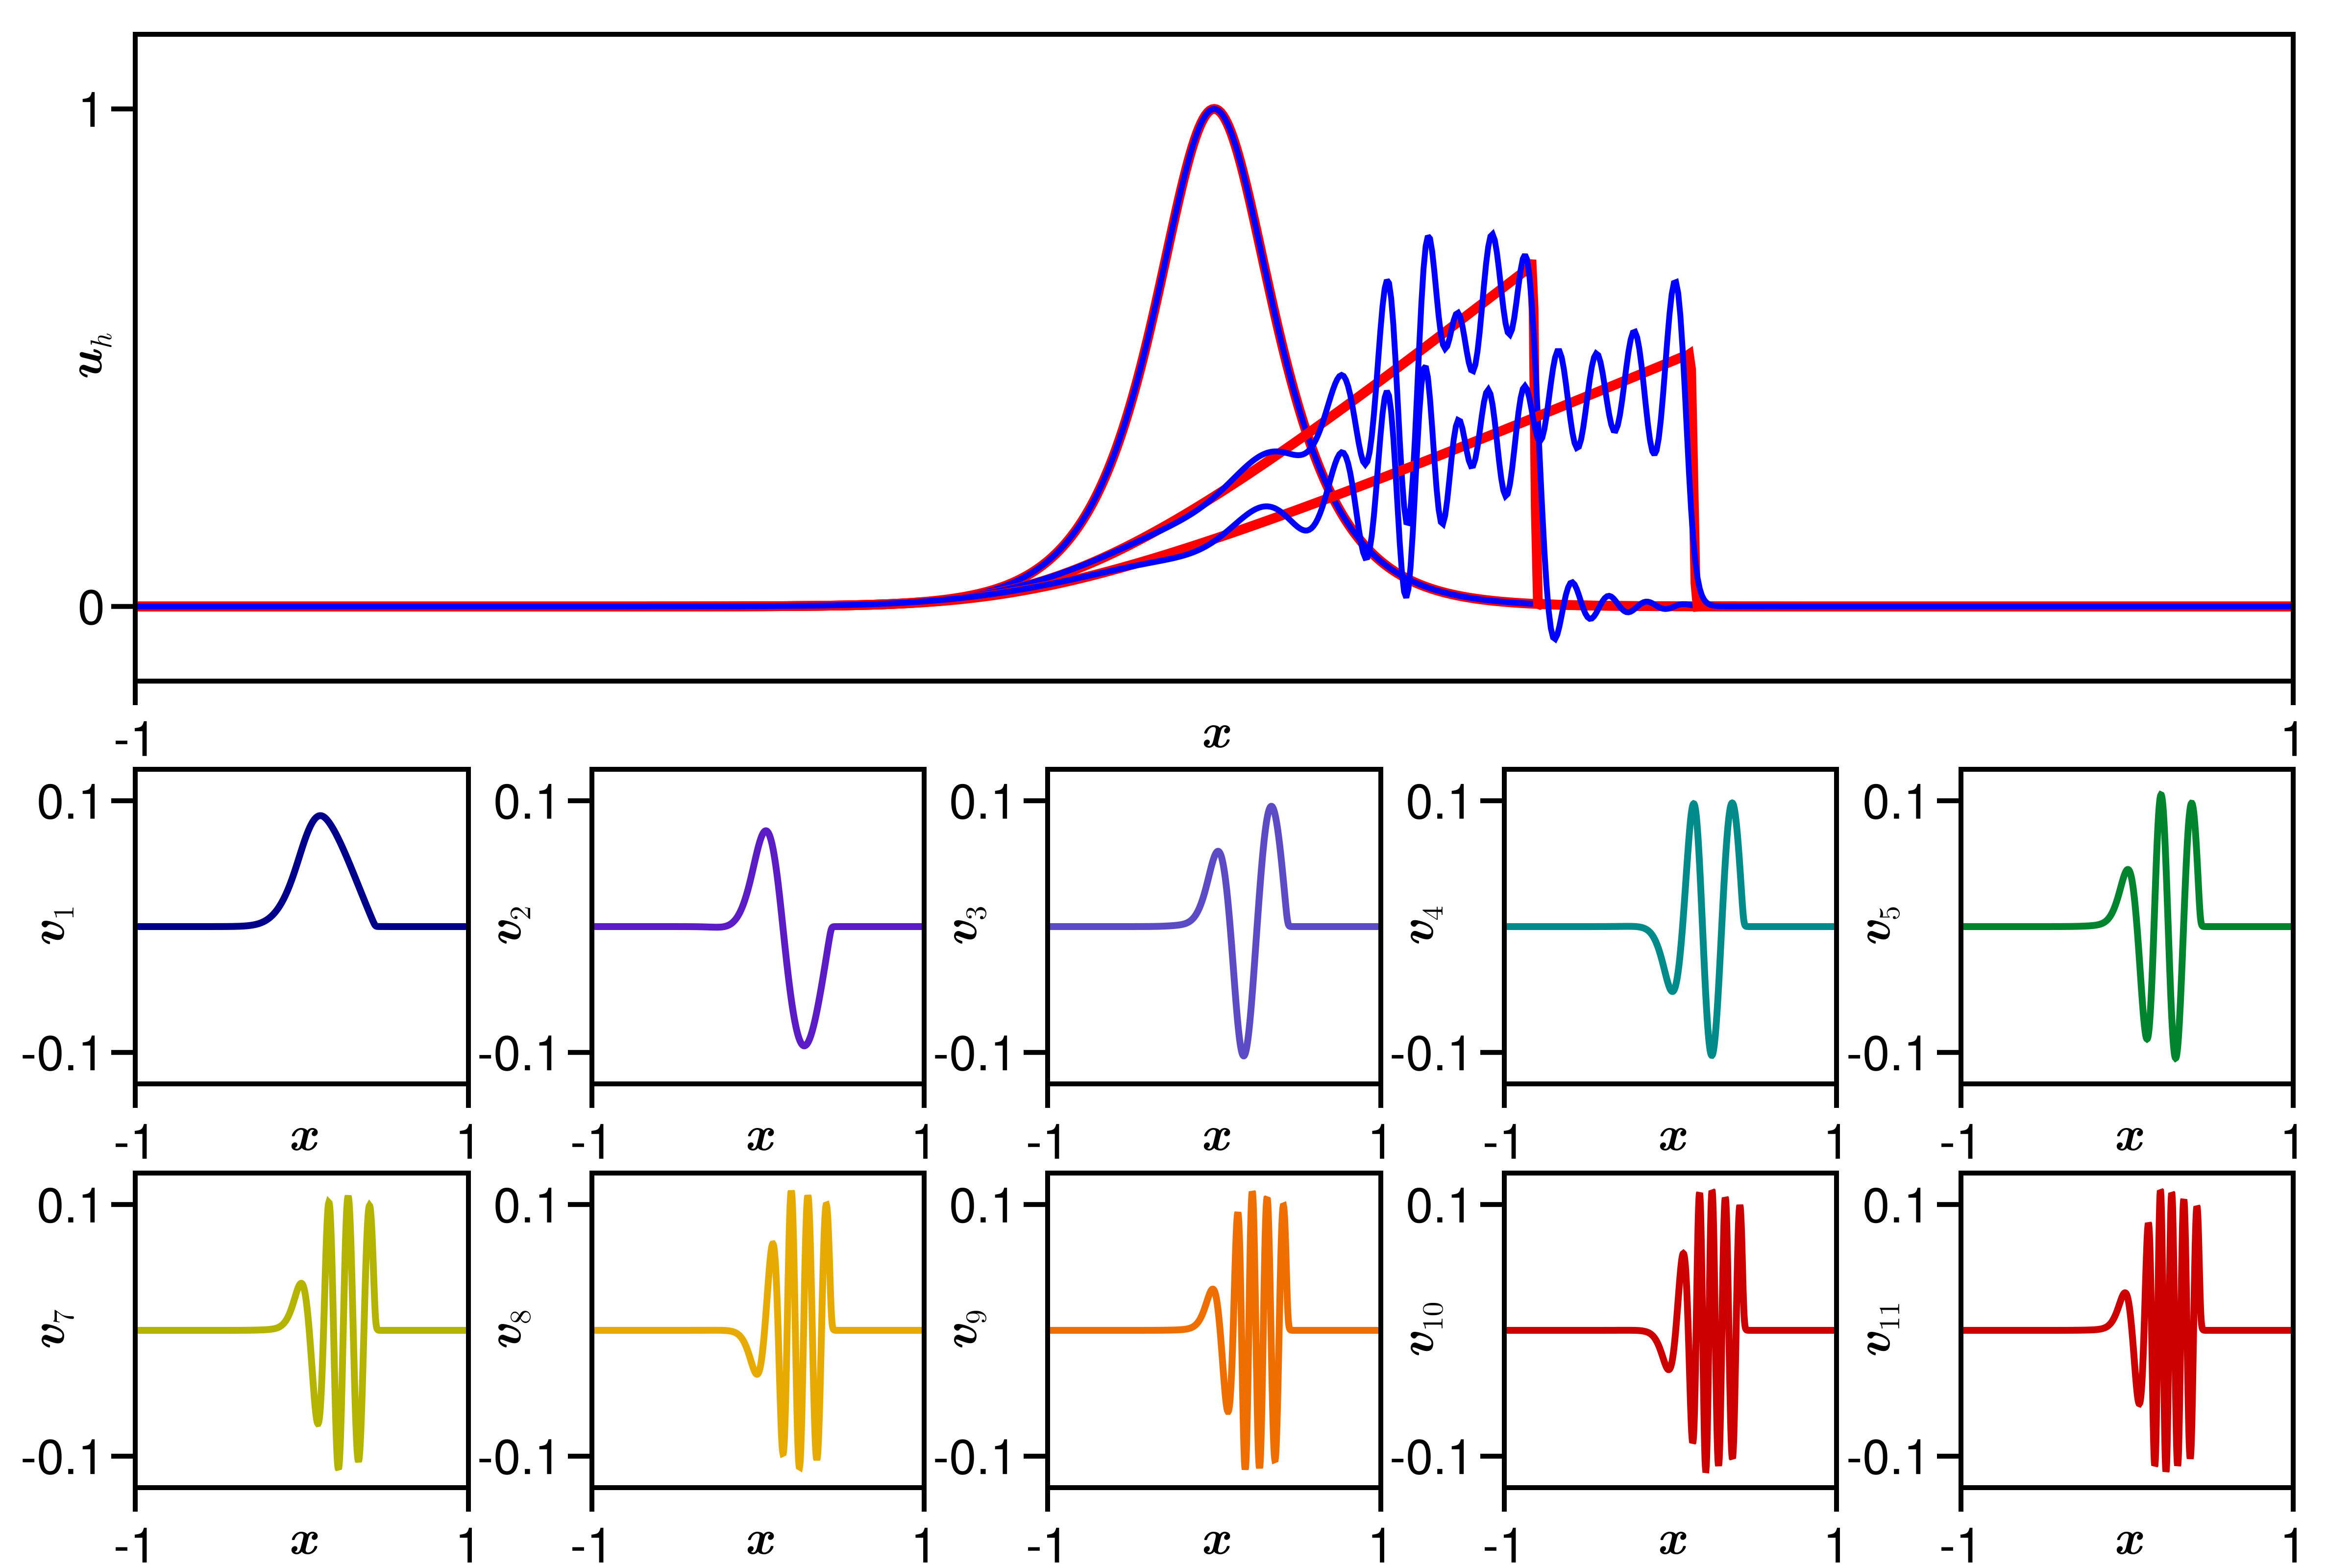
\includegraphics[keepaspectratio, width=0.75\textwidth]{../figures/fig:burgers_rom.png}
    \caption{\textbf{Top}: some solutions of the FOM (solid, red) and the ROM (dashed, blue) for parameter value $\mu = 0.02$.
             \textbf{Middle}: first $12$ of the total $N_{r}=22$ singular vectors spanning $\mathcal{R}_{h}$.}
    \label{fig:burgers_rom}
\end{figure}

As it is evinced from Figures \ref{fig:burgers_decay} and \ref{fig:burgers_rom}, not only traditional linear construction of the reduced manifold via POD is inefficient (at offline stage) for nonlinear hyperbolic problems, but the Galerkin projection also yields inaccurate reconstructions (at online stage) of the FOM.

\end{document}
